% Innehållet i Vasungavisor 2018
%
% Kapitel "Fafa Ska Sjung"

\begin{intersong}
\sffamily\bfseries\LARGE\centering{Fafa Ska Sjung}
	\begin{center}
		\vspace{10mm}
	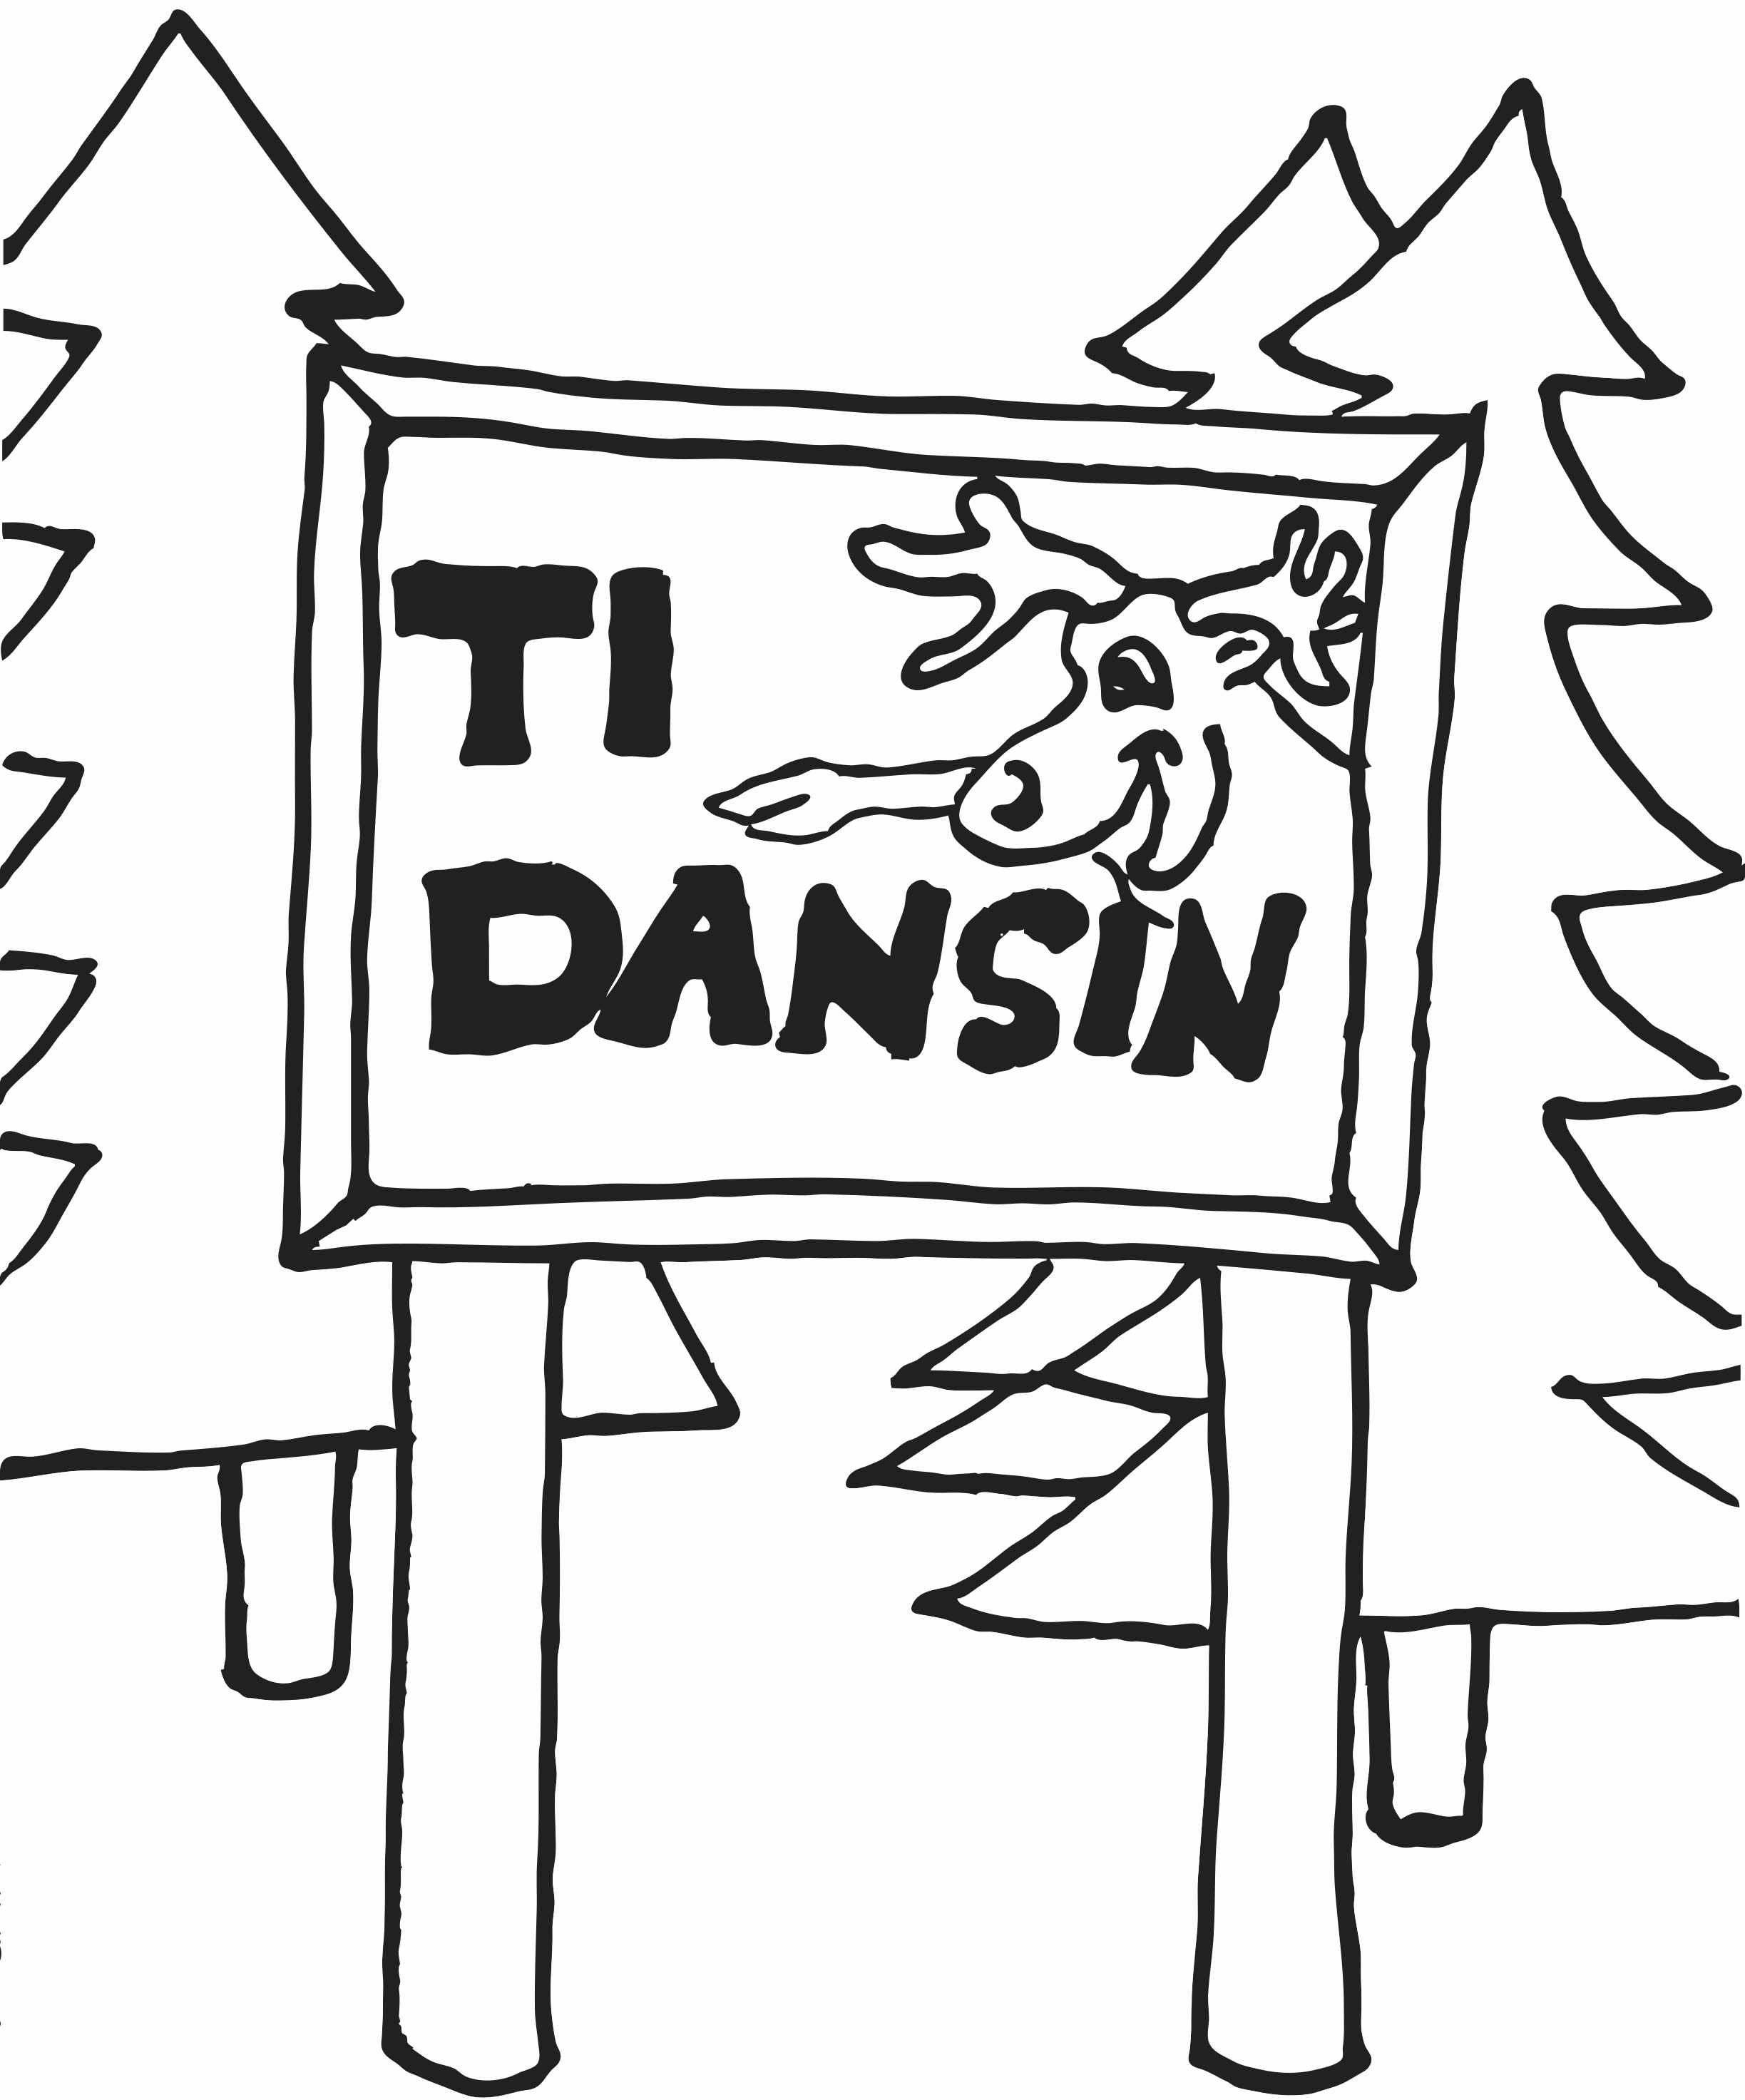
\includegraphics[width=0.9\textwidth]{../bilder/fardigabilder/BilderTillKapitel/tidansin.png}
\end{center} 
\end{intersong}
\sclearpage
% Sångtext till VN:s sångbok 2010.

% Denna fil kan användas som sådan, bara verserna,
% namnen och annan rådata behöver bytas ur fälten.
% Tecknet "%" markerar en kommentar som helt och 
% hållet ignoreras av programmet som läser filen.

\beginsong{In blåmåla plåtbåt}[ 		% Börja sången här
	by={Anders Teir},					% Författare
	sr={Proud Mary},					% Melodi
	index={Emel for åp ped ti Öjen}, 						% Alternativa
	index={Tusan, jäken, köm a stuli nöulon}]						% sångnamn
	

\beginverse*						% Börja vers
Emel for åp ped ti Öjen
markan i in burk å e mäitspö me.
Åp strandän bräivär slussin
stal an se in roddbåt
for ut i Kaskusånde å sku buri mäit.
Men höfstup vort an longvåt
i in blåmåla plåtbåt.
Tusan, jäken
köm a stuli nöulon?
\endverse							% Sluta vers

\beginverse*						% Börja vers
Emel kom ti plomp i fjälin
feg in rekti kalsup så an vela spy.
He smaka cellulosa,
smaka värr en dynjon.
Emel for ti båten som i seck med bly.
Men höfstup kom e titåt
in blåmåla plåtbåt.
Tusan, jäken
tennar kommer Folkline!
\endverse							% Sluta vers

\beginverse*						% Börja vers
Folkline tjuta me sirenin
å Emel dro di opp som in arin mört
Så tömd di ur an vattne,
å tömd i an na välkan.
Emel liva i å va itt ens na trött.
Ä notstup for an häimåt
i in blåmåla plåtbåt.
:,: Tusan, jäken
köm a stuli nöulon? :,:
\endverse							% Sluta vers
\endsong							% Sluta sång

\begin{intersong}
\includegraphics[scale=.4]{../bilder/in_blamala_platbat.png} 
\end{intersong}

\sclearpage
% Sångtext till VN:s sångbok 2018.

% Denna fil kan användas som sådan, bara verserna,
% namnen och annan rådata behöver bytas ur fälten.
% Tecknet "%" markerar en kommentar som helt och 
% hållet ignoreras av programmet som läser filen.

\beginsong{Kåtong fields}[ 		% Börja sången här
	by={Anders Teir},					% Författare
	sr={Cotton Fields},					% Melodi
	index={Josip va in litin, litin klepp}]						% sångnamn
	

\beginverse*						% Börja vers
Josip va in litin, litin klepp som bodd
naschtans i Kåtnäs lame mamm sin.
Han va blå, Kåtong-, Kåtongblå.
Han va ylak å skräik å råla ter an låg
i vaggon mitt i rume,
i en rekti Kåtongvagg där häim.
\endverse							% Sluta vers

\beginverse*						% Börja vers
Mamm hans sa: Kva je e nu fö rålas
näj nu tror ja nov vi flyttar jag å frassin.
Tu je blå, Kåtong-, Kåtongblå.
A så for on åp motorpede som e schtjitit
streck i Klockarbackan
å in rekti Kåtongfrass sat åp.
\endverse							% Sluta vers

\beginverse*						% Börja vers
Men just vör Bila jälma frassin
så e bar fö tjeljän ut i ditje,
i e slaskåt, gåråt Kåtongdik.
He va just tenn vör Kåtongbodän
fast i anna ditje neri backan
i e slaskåt, gåråt Kåtongdik.
\endverse							% Sluta vers
\endsong							% Sluta sång


\begin{intersong}
	\begin{center}
		\vspace{20mm}
		\includegraphics[width=7cm]{../bilder/katongfields.png} 
	\end{center}
\end{intersong}
% Innehållet i Vasungavisor 2018

\beginsong{Vååre i Pedäsi}[
  by={Erik Sundholm},
  sr={Vårvindar friska},
  index={Som förr om åårä}]
  
\beginverse*
Än som förr om åårä
kåmbär ååter våårä
blååsand ifrån än varmare zoon.
Taatsä ti dråppar
all skranglo tåppar
gröönskar på pälargoon.
Fågla ti vääsnas värr än di bruuk
tsänslona vaar så öim å så mjuuk.
Onga åm kvälda
sväittas ondi fällda
knälldär å foodrar struuk.
\endverse

\beginverse*
Kansje vi prooar
mang sårttäs skooar
fön e vaar tårtt på bakka än daag.
Snuuo ska bräkk ås
hoosto ska knäkk ås
bäinä vaar mjuuk å svaag.
Men om vi gaar åt Fäboda til
krååko ho slåår i stjye sin drill.
Takkona lambar
äinriisi dambar
tsänga vaar yyr å vill.
\endverse

\beginverse*
Driivona löisis
Remso ho pöisis
vattni hä stuuar upp i all diik.
Iisa ti blåkknar
pimplarä dråkknar
fast i än grunnän viik.
\newpage
Men saan ti nåågra som lämnar kvaar
bär uut motoorä siin som di haar.
Lägger döm i bååta
som är roti i nååta
puustar å svär å draar.
\endverse

\beginverse*
Daga vaar länger
nääträ vaar tränger
snaart siir a duuni runt uuta äld.
Hööger å hööger
soolä ho hänger
äin meeter minsta var kväld.
Gräsi hä fröudas räj vi var knuut
kuuddona röutar räj å vil uut.
Stinn vaar i haga
juuri ondi maga
böndrä vaar nöjd ti sluut.
\endverse
\endsong
\sclearpage
% Sångtext till VN:s sångbok 2018.

% Denna fil kan användas som sådan, bara verserna,
% namnen och annan rådata behöver bytas ur fälten.
% Tecknet "%" markerar en kommentar som helt och 
% hållet ignoreras av programmet som läser filen.

\beginsong{Astu-Mattas omvändelse}[					% Melodi
	index={Brännvini he e no ein krångloan vääto}]						% sångnamn
	

\beginverse*						% Börja vers
Brännvini he'e no ein krångloan vääto.
Mang gang he lagar ein i uusliheit å trääto.
Nooga måst an räkn ut ho mytji 'a tål
tå a' naangang styrker se me alkohål.
\endverse							% Sluta vers

\beginverse*						% Börja vers
Tå Astu-Matt pa va ti staan å hadd na mark i tasko,
så kåmb a alder heim om int an hadd naa i flasko.
Tjärndji ho bruuka taa i moot a ibland
halvvägs ti veiji mä språta i hand.
\endverse							% Sluta vers

\beginverse*						% Börja vers
Ein gang tå an ååter hadd ein fyllo se skaffa
Tjärndji byrja grobel yvi horleis ho sko straff a.
Gobbi låå å snarka på söötöra sett.
Tjärndji klädd tå ååv an så försiktit å nett.
\endverse							% Sluta vers

\beginverse*						% Börja vers
Så sest ho ner mä kläädre hans å byria sprätt å 
sööm om
varinda plagg så snääv å trang så knapt naan sko
drööm om.
Pyyla döm på gobbi såm i fyllo siin låå.
Lekst sist å såva i ein sjildan råå.
\endverse							% Sluta vers

\beginverse*						% Börja vers
Mot mårne tå a kvikkna till å byrja klarn i sinni,
så tjend a så i kroppi jyså kårve in i sjinni,
byrja roop ett tjärndji siin å ljuudi va så möör,
at hon sko kom å jälp a för a halder på å döör.
\endverse							% Sluta vers

\beginverse*						% Börja vers
Tjärndji djik ti sändji 'ans å roopa ``sööta gulli''
å jembra se å lååsta rååm å saa ``Va tu e svuldi
nu ha e entå gaai så ja så mang gang ha sagt'
så brännvini ha de ner på dööbeddi lagt.''
\endverse							% Sluta vers

\beginverse*						% Börja vers
Å gobbi saa att plåågona va stoor, å sluut va håppi.
Men kåmbä ja ifråån dehäär me liivi kvaar i kråppi
så låvar ja me hand på monn, å minns va ja seir,
ti alldär slepp ein brännviinsdråppo neir i strupi meid'.
\endverse							% Sluta vers

\beginverse*						% Börja vers
Tå ömsa tjärndji klääde ååv an, såm var vååt åv skumi
å linda döm i lakane å bar döm uut uur ryymi.
Sylma släfft å gobbi a djik opp på tridi daan.
Men han sko int ha trösta taa eins Håffmansdråppa
saan.
\endverse							% Sluta vers

\endsong							% Sluta sång
\begin{intersong}
\begin{center}
\includegraphics[width=4cm]{../bilder/brannvinsflaska.jpg} 
\end{center}
\end{intersong}
\sclearpage
% Sångtext till VN:s sångbok 2018.

% Denna fil kan användas som sådan, bara verserna,
% namnen och annan rådata behöver bytas ur fälten.
% Tecknet "%" markerar en kommentar som helt och 
% hållet ignoreras av programmet som läser filen.

\beginsong{Full i femton år}[ 		% Börja sången här
	by={Österbottnisk dryckesvisa},					% Författare
	sr={},					% Melodi
	index={Å ja ha vari full i femton år}]						% sångnamn
	


\beginverse*						% Börja vers
Å ja ha vari full i femton år
men int ha e nu satt na jävla spår
/: åp kråppin män, åp kråppin män
å lieävren täij e no å uutan såår.:/
\endverse							% Sluta vers

\beginverse*						% Börja vers
Om Alko höjer priserna i år
vi klarar alla kriserna gutår
/: fortfarande frånvarande
vi dricker nåt motsvarande gutår.:/
\endverse

\endsong							% Sluta sång
% Sångtext till VN:s sångbok 2018.

% Denna fil kan användas som sådan, bara verserna,
% namnen och annan rådata behöver bytas ur fälten.
% Tecknet "%" markerar en kommentar som helt och 
% hållet ignoreras av programmet som läser filen.

\beginsong{Noppåviiså}[ 		% Börja sången här
	by={Fritiof Remell},					% Författare
	sr={},					% Melodi
	index={Hälsninga har ja ifrån Linnuspera}, 						% Alternativa
	index={Rump rump rumpeliraa}]						% sångnamn
	

\beginverse*						% Börja vers
Hälsninga har ja ifrån Linnuspera
ter vi pedigreerar.
Hannes å ja tsöft varsin koddå en da
å vi kontrolleera:
Miin va en noppå, hä juså kukkå
tå får di koma mä va noppona di haar.
He too åpp grinda, så mytsi e hinda
tå foor ja strax ti en djuurlääkar.
A han sa såstee. ``Tu sko booda dsee
nu å tå en lillan suup såstee''.
Ja to rååda fö goo å ein knårrkopp droo
heila noppå in i sömnes roo.
Saan så vaknast e åpp, vaalt ti kåhmelå
håksa vingel ååv i illdsäälå,
men he jälpa braa, för he såå int naa
vartsin grinda eller klinkkona.
\endverse							% Sluta vers

\beginchorus
Rump, rump, rumpeliraa
söjs er ti nopponaa.
Ja pa int vaal ill ut å åppstållt ja
en noppå e braa til haa.
\endchorus

\beginverse*						% Börja vers
Ni ska int tro e a viri skruuft
för he tappa jämtrå.
En tiid så böula he å hadd så druuft,
håksa vaal ti kräntså.
Men ja tänkt jysså, hä fol int bysså
he kan jo jämter mä va jämtrå e kvaar.
Ja foor tii staan, å ter tsöft ja saan
ti gröön pare brillona så noppå nu har.
He er rooli me glasögona he tror et
alltihop e gröönfoodrä.
Tå ja bruukar still tärttis he måår iil
tycker ja he boodi noo räck till.
Ja bruukar haa Jorvas kaakonaa
tömte rovvonaa å pååponaa,
men så hååkon too he får alder noo
juså Majaback koddå uutan roo.
\endverse	

\beginchorus		
Rump, rump...
\endchorus					% Sluta vers

\beginverse*						% Börja vers
Ni kan int tro va he er löös ti målk,
hur e dseer i stsuulå.
He kåmber bara juså an sko pålk,
he bäst jer å imillan Uulå.
lnt naasås djuura haar toko juura,
tå får di koma mä va juura di haar.
Om man drar ein gang, komber e
fleir gang, å ni kan int troo tokan
romppå e haar.
Juså svängdöre å på gångjääne,
viitsis bort, så int e sloiskar naa.
Nu får kvinnfålttsi mytsi båter ti
hald he romppå bårt från möjkhinttsi.
Nu ska int an träng, ha e täär å häng,
he ha noo hängd teer rei laagom läng
å betyydelse har e alltiili. Stämber
Korp-Matt saa tacksägelsi.
\endverse	

\beginchorus	
Rump, rump...
\endchorus						% Sluta vers

\endsong							% Sluta sång




\begin{intersong}
\begin{center}
\includegraphics[width=5cm]{../bilder/natur.jpg} 
\end{center}
\end{intersong}
\sclearpage
% Sångtext till VN:s sångbok 2018.

% Denna fil kan användas som sådan, bara verserna,
% namnen och annan rådata behöver bytas ur fälten.
% Tecknet "%" markerar en kommentar som helt och 
% hållet ignoreras av programmet som läser filen.

\beginsong{Grannas skithus}[ 		% Börja sången här					% Författare
	sr={Byssan lull},					% Melodi
	index={Grannas skithus ha raka ikull}]						% sångnamn
	


\beginverse*						% Börja vers
Grannas skithus ha raka ikull,
å vårat he står tär å lytar.
Bäter ti ha ett rokoe eitt,
än ti vaa rikti ytan.
\endverse							% Sluta vers

\beginchorus
Fafa ska sjung,
fafa ska sjung,
fafa ska sjung för lill tollon sin.
\endchorus

\beginverse*						% Börja vers
Tattarn ha stuli tupplotji vårt,
å potton ho gistnar på gärdin. 
He finns så myki som
e sorgeligt å svårt,
he finns så myki sorger i världin.
\endverse		
\beginchorus
Fafa ska sjung...
\endchorus					% Sluta vers

\beginverse*						% Börja vers
Tänkin å undrin va öid he sku va
om eldin sku slokin i spisin.
Å int sku vi kun kok,
å int sku vi kun steik,
å int sku vi få mat åt grisin.
\endverse		
\beginchorus
Fafa ska sjung...
\endchorus					% Sluta vers


%Extra vers jag hittade..
%Byssan Lull, kaki byssorna full,
%så knyter vi till om kneina.
%Så släpper vi opp,
%och så rinner he neir,
%å då blir du kakiger om beina.
%Fafa ska sjung...




\endsong							% Sluta sång
\sclearpage
% Sångtext till VN:s sångbok 2010.

% Denna fil kan användas som sådan, bara verserna,
% namnen och annan rådata behöver bytas ur fälten.
% Tecknet "%" markerar en kommentar som helt och 
% hållet ignoreras av programmet som läser filen.

\beginsong{Heimani i skick}[ 		% Börja sången här
	by={KAJ}]						% sångnamn
	

\beginverse*						% Börja vers
Vi e gladeligen under paviljongens tak
Sko damerna i salen vilja skaka på sin bak

Höftrin rör ni smidigt liksom ny escortins servo
Att säg att hipsan ljuger he sko va att va ett pervo

UF ordnar disco å ikväll ere fullt hus
Strobolightsin vår den e ti vardags arbetsljus

Pängan skyltar pojkan me men brudan den får nåog
den kombär heim me oss fö vi har tjugo hektar skåog
\endverse							% Sluta vers

\beginchorus
Att dem int föstår att man itt får brudar me
Ti skryt om märkesjeans å BMW
He enda som funkar om man vill få heim in flick
E att man har brysthår å heimani i skick
\endchorus

\beginverse*						% Börja vers
E spelas dunka dunka och rivig rock n'roll
Som tå fammo va på dansin fast i version två punkt noll

UF dom har slutat handla svindyr sprit från alko
Hädanefter görs brännvinet kostnadsfritt på talko

I paviljongens bar så säljs det fjolårstrip å kex
från övranvåningen så hörs ett tydligt ljud av skratt 

Säg itt att do e pengakarl tå anses do som e lame
Men berättar do om föusi det gar itt do eismend heim
\endverse							% Sluta vers

\beginchorus
Att dem int föstår att man itt får brudar me
Ti skryt om märkesjeans å BMW
He enda som funkar om man vill få heim in flick
E att man har brysthår å heimani i skick
\endchorus

\beginverse*						% Börja vers
Jå eje precis såde e je
Man ska va bond elo skogsägare 

Om do har e i de men do veit it vann
Bli en man så fåort do kan

Om do känder do e i en svacko,
Ta flanellskjåorton och bombarjackon

E je såde do hamnar högst på toppen
Å skaffar brudar i Österbotten

Men do kanski e ejsmend å fundärar på na
Ska do va på elo spel svårfånga
Men e je int na skillna bara do har
Duktit me bryysthår å nager hektar
\endverse							% Sluta vers

\beginchorus
Att dem int föstår att man itt får brudar me
Ti skryt om märkesjeans å BMW
He enda som funkar om man vill få heim in flick
E att man har brysthår å heimani i skick
\endchorus

\beginchorus
Att dem int föstår att man itt får brudar me
Ti skryt om märkesjeans å pappos BMW
He enda som funkar om man vill få heim in flick
E att man har brysthår å heimani i skick
\endchorus

\endsong							% Sluta sång
\begin{intersong}
	\begin{center}
		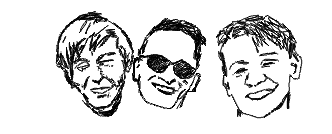
\includegraphics[width=0.75\textwidth]{../bilder/fardigabilder/CamillasFardigaBilder/humorgruppenKAJ.png} 
	\end{center}
\end{intersong}
% Sångtext till VN:s sångbok 2018.

% Denna fil kan användas som sådan, bara verserna,
% namnen och annan rådata behöver bytas ur fälten.
% Tecknet "%" markerar en kommentar som helt och 
% hållet ignoreras av programmet som läser filen.

\beginsong{Dehär e min by}[ 		% Börja sången här
	by={KAJ}]						% sångnamn
	

\beginverse*						% Börja vers
Gråa lador, gula fält
He e he enda ja naingang ha känt
Gålan röd å knutan vit
He e he enda ja naingang ha sitt

Å ja veit, att it e låter så bedrövlit
Å ja veit, att ja har allt som e behövlit
Men fast ja veit, allt ede
Så har ja it na ti jämför me
\endverse							% Sluta vers

\beginchorus
Dehär e mitt heim
dehär e min by 
Ja sko it byt an måot in nyy
Ja känder all föussin
å bakanett knöussin
ere bara massa sly
\endchorus

\beginverse*						% Börja vers
Ja ha drömd, om ett ställ
Tä man får va se själv å it måst klä se i flanell
Ett paradis tär man får välg
Mellan meir än ti stick sockor, elo styck in älg

Ja inom mig, tär ha e väckts ett hopp
Om ett liv me meir, än bara päror å kalops
\endverse							% Sluta vers

\beginchorus
Dehär e mitt heim
dehär e min by 
Om ja sko byt an måot in nyy
Tå sko ja slipp föussin
Å bakanett knöussin
sko ja sii en nyan vy
\endchorus

\beginverse*						% Börja vers
Me öppna landskap å oändliga hav
Utan talko å utan krav
Tär itt allt handlar om blåbärin
Tär ja sko pass in

Ja veit it va ja vill
Va ska ja ta me till
E finns jo itt na lätt svar på de här
Fast ja sko jär rätt 
så blir e heilt feil på na sätt
Åååh va ska ja jär
\endverse							% Sluta vers

\beginchorus
Dehär e mitt heim
dehär e min by 
Ja sko it byt an måot in nyy
Men ja ha sitt all föussin
å bakanett knöussin
Finns e meir än bara sly
\endchorus

\beginverse*						% Börja vers
E finns na som drar
å nainting som halder me kvar
Ja sko konn fly

Papp sko få plock sina egna bär
\endverse							% Sluta vers

\textnote{Även denna sång är publicerad med tillstånd av KAJ. Tacohej!}

\endsong							% Sluta sång
\sclearpage
% Innehållet i Vasungavisor 2018

\beginsong{Isoo-Antti ja Rannanjärvi}[
	by={},
	sr={}]

\beginverse*
Isoo-Antti ja Rannanjärvi
ne jutteli kahren kesken:
Tapa sinä Kauhavan ruma vallesmanni,
niin minä nain sen komian lesken.
\endverse

\beginverse*
Isoo-Antti oli ensimmäänen
ja Rannanjärvi oli toinen,
Pukkilan Jaska se Kauhavalta
oli kolmas samanmoinen.
\endverse

\beginverse*
Sitten on piru, sano Rannanjärvi,
jos minä miestä pelkän;
tervastampulla kuonon päälle
ja teräksellä pitkin selkää.
\endverse

\beginverse*
Vaasan veri ei vapise,
eikä Kauhavan rauta ruostu;
niskasta kiinni ja puukoolla selkähän,
jonsei se muutoon suostu.
\endverse

\beginverse*
Ensin ne portahat särjettiin
ja sitten vasta muuri;
Isoo-Antti se erellä meni,
joka joukosta oli suurin.
\endverse

\beginverse*
Ei saa laulaa Rannanjärvestä,
Rannanjärvi on kuollu.
Rannanjärven hauralle
on marmorikivi tuotu.
\endverse
\endsong
%% Sångtext till VN:s sångbok 2018.

% Denna fil kan användas som sådan, bara verserna,
% namnen och annan rådata behöver bytas ur fälten.
% Tecknet "%" markerar en kommentar som helt och 
% hållet ignoreras av programmet som läser filen.

\beginsong{NTM}[ 		% Börja sången här
	by={Johan Gullmets},					% Författare
	sr={TNT},					% Melodi
	index={Si me svättas kvalin da}, 						% Alternativa
	index={Ja je åp NTM}]						% sångnamn
	

\beginverse*						% Börja vers
Si me svättas kvalin da
åp Närpes trä och Metall
tier så sliter jag me ploåtin
om et väit kva ja säir.

Netchin brudar runt om mieg
skådar tå ja sloår
har itt nain pistol
har itt nain kniv
men in hamar oåv stoål.
\endverse							% Sluta vers

\beginchorus
Ja je åp NTM
me in hamar oåv stål.
NTM
he ligger i Buöle.
NTM
å tier drecker di uöle.
NTM
si tå ja sloår.
\endchorus

\beginverse*						% Börja vers
Stjiti, ylak, åp grymt humyör
kvinnor vill ha mieg
från Närko komber di å skoåd
hör an ska arbet.

Ta hit dotren, elå fruen
lies opp dönan å spring fö tett liv
fö snart je dajin slut
å karin släpper di ut.
\endverse							% Sluta vers

\beginchorus
Ja je åp NTM
me in hamar oåv stål.
NTM
he ligger i Buöle.
NTM
å tier drecker di uöle.
NTM
di lagar sopbilan.
NTM
som gar hondra milan.
NTM
di har stora hallar.
NTM
å di har stora ballar.
NTM
si tå ja sloår.
\endchorus

\endsong							% Sluta sång


